
\documentclass[14pt]{article}
\usepackage{extsizes}
\usepackage[english]{babel}
\usepackage[a4paper, top=3.5cm, bottom=2.5cm,left=3cm,right=3cm,marginparwidth=2cm]{geometry} % see geometry.pdf on how to lay out the page. There's lots.
\geometry{a4paper} % or letter or a5paper or ... etc
% \geometry{landscape} % rotated page geometry

% See the ``Article customise'' template for come common customisations
\usepackage{graphicx}
\graphicspath{ {./images/} }

\usepackage[colorlinks=true, allcolors=blue]{hyperref}
\usepackage{listings}
\lstdefinelanguage{JavaScript}{
  keywords={typeof, new, true, false, catch, function, return, null, catch, switch, var, if, in, while, do, else, case, break},
  keywordstyle=\color{blue}\bfseries,
  ndkeywords={class, export, boolean, throw, implements, import, this},
  ndkeywordstyle=\color{darkgray}\bfseries,
  identifierstyle=\color{black},
  sensitive=false,
  comment=[l]{//},
  morecomment=[s]{/*}{*/},
  commentstyle=\color{purple}\ttfamily,
  stringstyle=\color{red}\ttfamily,
  morestring=[b]',
  morestring=[b]"
}

\lstset{
    language=JavaScript,
    basicstyle=\ttfamily\small,
    aboveskip={1.0\baselineskip},
    belowskip={1.0\baselineskip},
    columns=fixed,
    extendedchars=true,
    breaklines=true,
    tabsize=4,
    prebreak=\raisebox{0ex}[0ex][0ex]{\ensuremath{\hookleftarrow}},
    frame=lines,
    showtabs=false,
    showspaces=false,
    showstringspaces=false,
    keywordstyle=\color[rgb]{0.627,0.126,0.941},
    commentstyle=\color[rgb]{0.133,0.545,0.133},
    stringstyle=\color[rgb]{01,0,0},
    numbers=left,
    numberstyle=\small,
    stepnumber=1,
    numbersep=10pt,
    captionpos=t,
    escapeinside={\%*}{*)}
}


\title{Final Project Report}
\author{Federico Perotto, 1701738}
\date{} % delete this line to display the current date

%%% BEGIN DOCUMENT
\begin{document}

\maketitle

\tableofcontents
\newpage

\section{Abstract}
This project is a minigame, where the objective is to turn off all 4 lights before the timer runs out. The timer starts when the first light is turned off, and if it reaches 35 seconds, all the lights turn back on.
The W and S key are used to move along the z axis, while the A and D keys are use to move along the x axis. The E key can be used to turn off a light if the character is close enough to it.

\section{Environment}
The project was developed mainly with \textbf{Three.js}, which is a javascript library meant to render 3D graphics in web browsers through the usage of WebGL. It provides multiple intuitive and easy to use methods to implement cameras, objects, geometries, textures, models, lights and more. On top of Three.js, \textbf{Tween.js} was also used to implement smooth animations and the tweening betweeen keyframes.

\section{Libraries, tools and models}
\subsection{Libraries}
The only libraries used are the already cited above Three.js and Tween.js, but Three.js provides multiple tools to ease development, like camera controls, texture loaders, model loaders and performance trackers.

\subsection{Tools}
\begin{itemize}
	\item \textbf{Stats:} A useful tool provided by Three.js that implements a small widget to keep track of the application's performance.
	\item \textbf{GLTFLoader:}  A tool provided by Three.js that allows for the loading of 3D models in the \textit{gltf} format (the one preferred by WebGL), with their structure, mesh, textures, and animations. In this project it is used to load the character model ( \textit{RiggedFigure.glb}) and the torch model ( \textit{wall\_torch.gltf}).
	\item \textbf{TextureLoader:} Another loader, this time for textures and images. It loads 3 textures in total, one for the floor ( \textit{dungeon\_floor.jpg}), one for the walls ( \textit{drywall.jpg}) and one for the rotating columns ( \textit{mattoni.jpg}).
	\item \textbf{LoadingManager:} A manager for the loaders, used to make sure that all the assets are loaded before creating the scene and running the animation loop.
	\item \textbf{OrbitControls:} Another tool provided by Three.js which allows the user to control the camera with the mouse and arrow keys. It is used to allow the player to look around and better see the map.
\end{itemize}

\bigskip
\subsection{Models}

\begin{tabular}{p{13.5cm}p{2cm}}
	 \minipage{13cm} \renewcommand{\arraystretch}{1} \begin{tabular}{@{}p{2mm}p{11.5cm}@{}} • & \textbf{RiggedFigure.glb:} A simple rigged 3d model with no textures from the \href{https://github.com/KhronosGroup/glTF-Sample-Models/tree/master/2.0/RiggedFigure}{Khronos Group gltf sample models.} Its hierarchical structure is composed of 19  elements, most of which are animated with tween.js.\end{tabular}\endminipage 
 \minipage{2cm}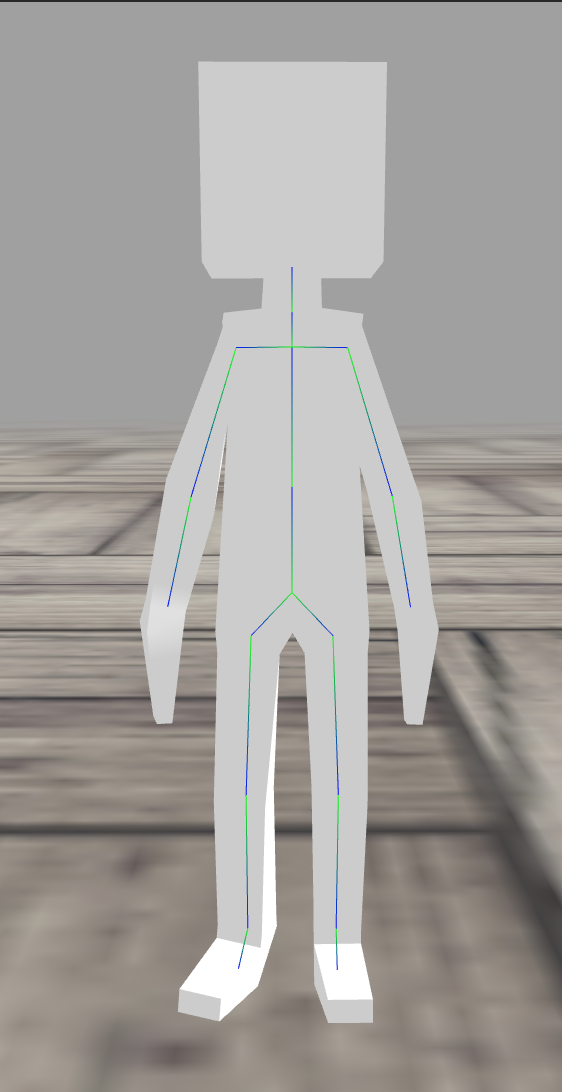
\includegraphics[width=2cm]{model.png}\endminipage
 \end{tabular}
 
 \bigskip
 
 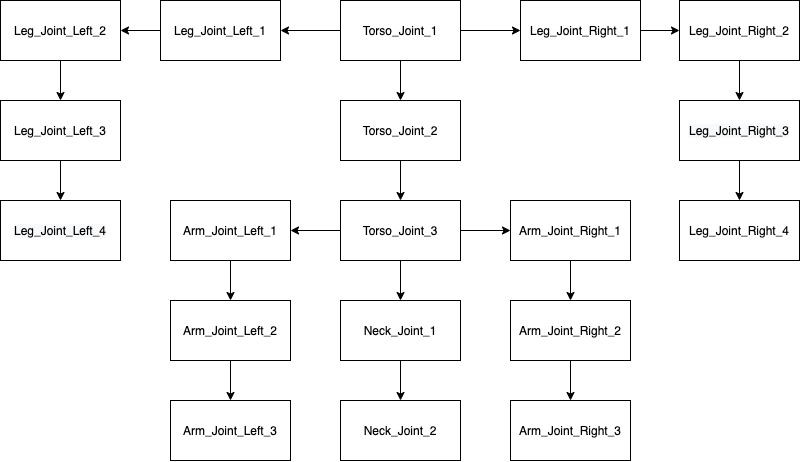
\includegraphics[width = 13cm]{hs.jpg}
 
 \bigskip
 \begin{tabular}{p{13.5cm}p{2cm}}
	 \minipage{13cm} \renewcommand{\arraystretch}{1} \begin{tabular}{@{}p{2mm}p{11.5cm}@{}} • & \textbf{wall\_torch.gltf} A more complex wall torch model with textures, downloaded royalty-free from \href{https://sketchfab.com/3d-models/wall-torch-7ede870750ba4831b6cb4669bb1c58c0}{sketchfab.}\end{tabular}\endminipage 
 \minipage{2cm}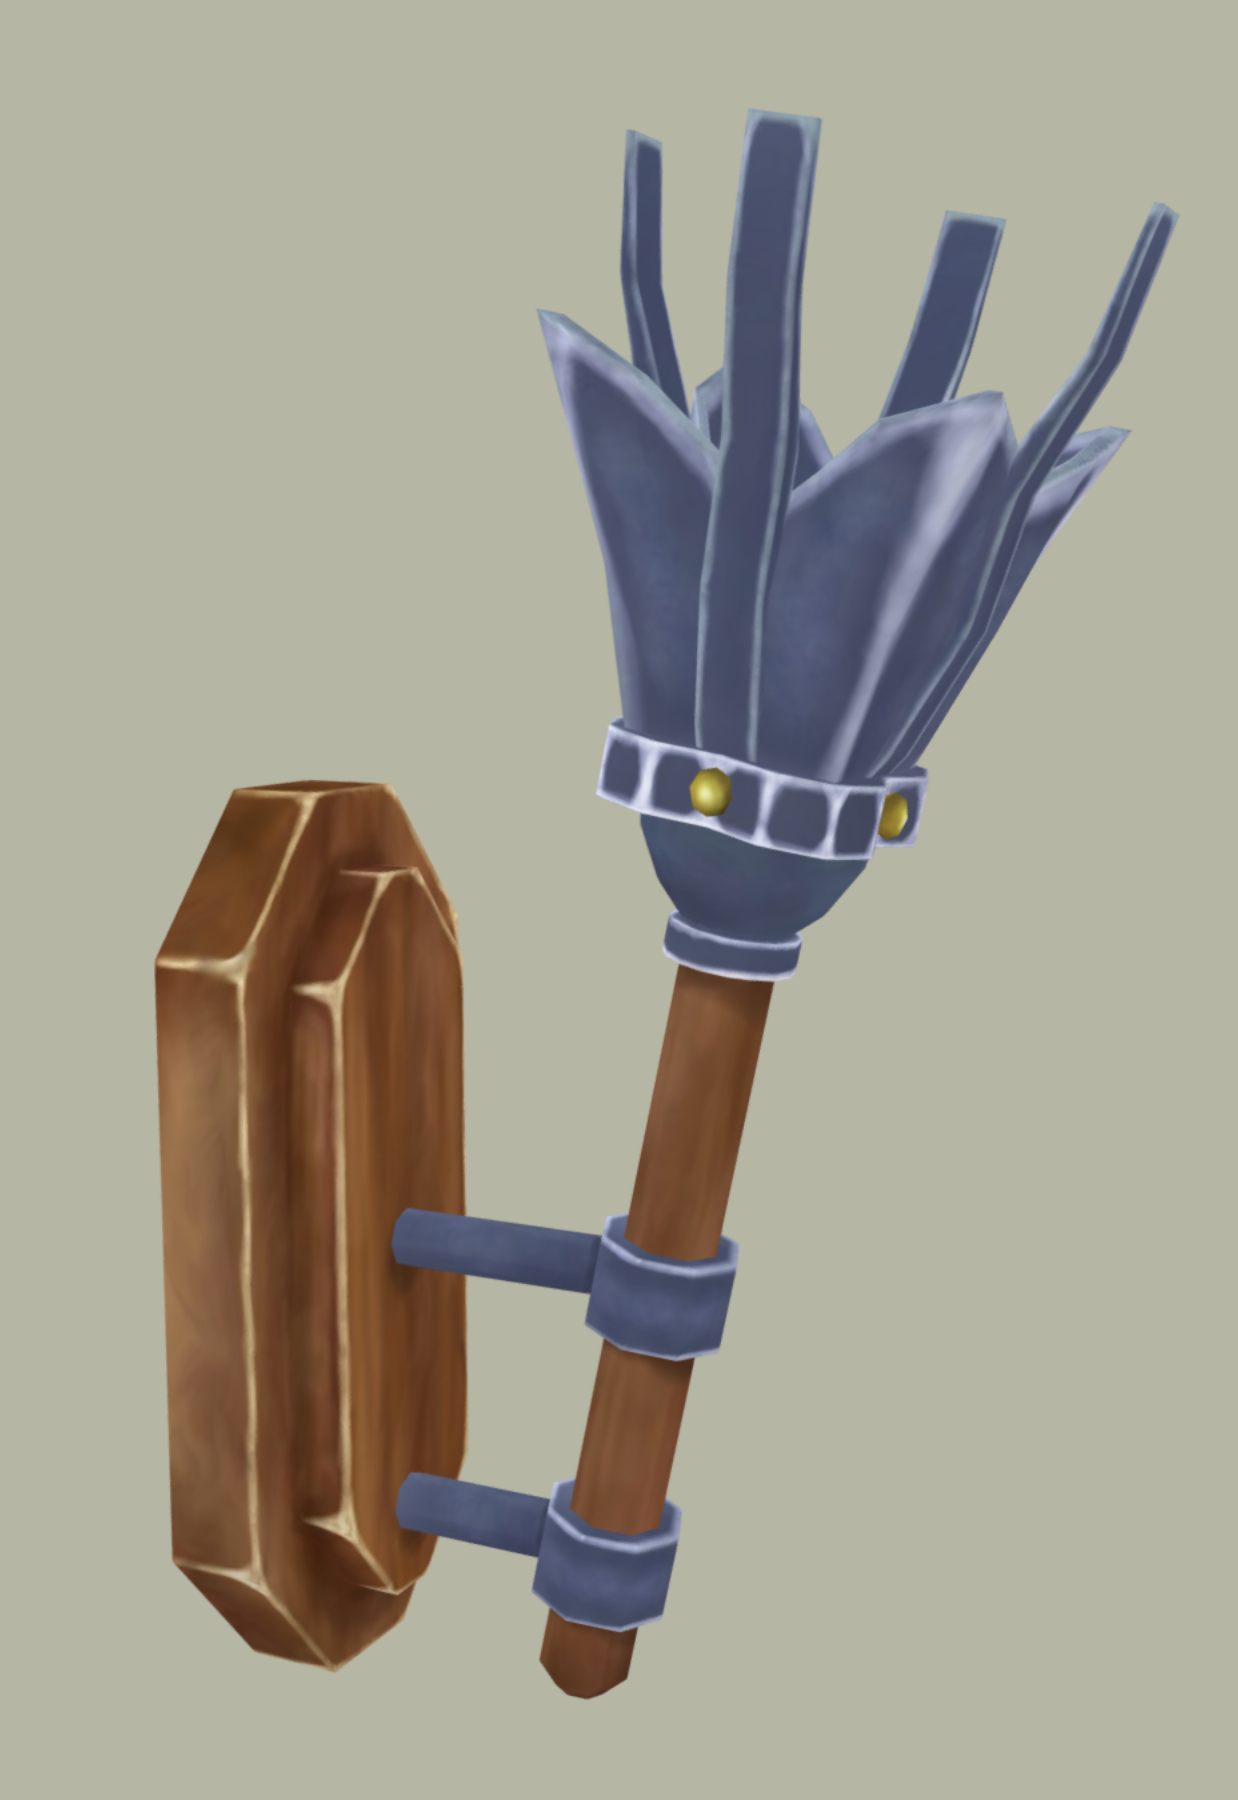
\includegraphics[width=2cm]{torch.png}\endminipage
 \end{tabular}



\section{Technical Aspects}
\subsection{Setup}
The LoadingManager waits for all of the assets to be loaded before setting up the Three.js scene. The  \textit{onProgress()} callback function of the LoadingManager is used to update the loading bar in the loading screen, while the  \textit{onLoad()} callback function is used to call the  \textit{init()} function, which sets up the scene.
\\


The  \textit{init()} function sets up the level by adding all the geometries, the textures, the models and the lights,  and sets all their respective properties, before calling the animation loop.
\\

The geometries are added to an array of "collidable" objects, which is used to check for collision with the model. The collision checking is based on 4 raycasters that originate from the model position and at each frame check if they are touching any of the "collidable" objects in order to prevent the player from walking inside of them.
\\


In the scene there is a hemisphere light and 4 point lights. The point lights are meant to represent the torches flames, which is why they are orange. Due to poor performances with how Three.js computes shadows (especially for point lights), I have decided to set the castShadow property of the point light to false.
\\


The two rotating pillars have a torch model each as a children, and each of these torch has a point light as a children. So once they have been positioned relative to their parents, the rotating column will automatically update the position of the torch and the light.


\subsection{Event Listeners}
Event listeners are used to detect whenever a key is pressed or released. The W, A, S and D keys control movement along the x and z axis (camera orientation doesn't influence which axis the keys control). 

These events are also responsible for calling the  \textit{run()} function, the  \textit{resetModelStance()} function and the functions that make the model turn.

\subsection{Movement}
The actual position of the character is changed in the render loop, while the running animation, as well as the turning animations and the  \textit{resetModelStance()} function utilize Tween.js.
\\

The run() function contains the movement animation logic, which exploits Tween.js. The model moves his arms and legs alternatively to emulate a simplified running animation: both the arms and the legs move ahead and back alternatively and are diagonally aligned. So if the left arm is ahead, the right arm is behind, the right leg is ahead and the left leg is behind. 
\\

The movement of the arms and the legs is tweened between 4 positions (keyframes) that use the  \textit{onComplete()} callback function to make sure they execute in the correct order and that each sub-animation finishes before starting the next one.

\bigbreak
\begin{lstlisting}[language=JavaScript, caption={Running animation function for the left side of the body}]
	function run(){
			
		var tween_start_L = new TWEEN.Tween([leg_joint_L_1.rotation, leg_joint_L_2.rotation, arm_joint_L_1.rotation, arm_joint_L_2.rotation]).to([{x:0.312, y: 0.591, z: -3.108}, {x:-1.645, y:-0.005, z:0.614}, {x: 2.903, y: -1.255, z: -2.391}, {x: 0.116, y: 0.268, z: 0.485}], 500).start();

		tween_start_L.onComplete(function(){
			var tween_middle_L = new TWEEN.Tween([leg_joint_L_1.rotation, leg_joint_L_2.rotation, arm_joint_L_1.rotation, arm_joint_L_2.rotation]).to([{x: 0.912, y: 0.591, z: -3.108}, {x:-0.405, y: 0.587, z: 0.192}, {x: 2.903, y: -1.255, z: -1.641}, {x: 0.116, y: 0.268, z: 0.068}], 300).start();
					
			tween_middle_L.onComplete(function(){
				var tween_end_L = new TWEEN.Tween([leg_joint_L_1.rotation, leg_joint_L_2.rotation, arm_joint_L_1.rotation, arm_joint_L_2.rotation]).to([{x: 2.512, y: 0.591, z: -3.108}, {x: -0.847, y: 0.465, z: 0.417}, {x:2.903, y: -1.255, z: -1.041}, {x: -0.084, y: -0.131, z: 1.367}], 700).start();
							
				tween_end_L.onComplete(function(){
					var tween_reset_L = new TWEEN.Tween([arm_joint_L_1.rotation, arm_joint_L_2.rotation]).to([{x: 2.903, y: -1.255, z: -1.641}, {x:0.116, y: 0.268, z: 0.068}], 200).start();
								running = false;
				});
			});
		});
	};
			\end{lstlisting}

\subsection{Animation Loop}
The  \textit{animate()} function, before requesting the next frame, checks if the win condition has been met. 

If so, it stops the loop and builds a victory screen, which has a button to restart the minigame; if the win condition hasn't been met, it requests the next frame, and then take cares of rotating the columns and moving the model and the camera. 
\\

The function also implements a rudimentary collision checking system that checks for collisions by casting 4 rays from the model towards the positive x and z and towards the negative x and z. If it detects a collision of any of the rays with one of the "collidable" objects, it prevents the movement by setting the  \textit{move\_direction} to false, where  \textit{direction} is determined by which ray detects a collision.
\\

Finally the function checks if the timer is started and if it has gone over 35 seconds, in which case the lights get turned back on.
 
\bigskip


  
\section{Interactions}
The first interaction is obviously the character movement with the use of the keyboard. 
Each of the W, A, S and D key, if no other key is pressed and if the running flag is set to false, changes the running flag value to true, and the  \textit{move\_direction} flag to true, where  \textit{direction} is determined by the key that is pressed. Then the event makes sure that the character is facing in the right direction, and if not it corrects its rotation. Finally the run() animation is called.
\\

Whenever a key is released, it fires a  \textit{keyUp} event, which resets all the flags associated with that key to false, the running flag to false and resets the model position to its default stance.
\\

The other main interaction is the ability to turn off the torches (or their point lights to be exact). 
When all the lights are created, they get put in an array, and when the E key is pressed, its  \textit{keyDown} event iterates over the lights in the array, it gets their position relative to the world origin and compares it to the model position. If it finds a light that is close enough, it turns that light off and starts the timer. 

\end{document}








